\begin{abstract}
Since the beginning of AI research, the study on one of its core
component, graph search, has long focused on how to guide it using the
heuristic estimate and how to improve the estimates.  One thing that has
been out of focus is the study on tiebreaking, or how to \emph{directly}
improve the search performance on a plateau without changing the
heuristics nor search algorithms.  Such techniques should be done
without help of additional information from the heuristics because
theoretically there is some point that the heuristics cannot be improved
any more while the plateau is still exponentially large.

In this paper, we investigate and improve tiebreaking strategies for
 optimising search using A* and satisficing search using GBFS.
For A*, we first experimentally analyze the performance of common tiebreaking strategies that break ties according to the heuristic value of the nodes.
We find that tiebreaking has a significant impact on search algorithm performance when there are zero-cost operators that induce large plateau regions in the search space.
Next we develop a new framework for tiebreaking based on a depth metric which
 measures the distance from the entrance to the plateau, and propose a new, diversifying strategy which significantly outperforms standard strategies on domains with zero-cost actions. 

We also apply the same strategy to GBFS for satisficing search, where
 currently no obvious tiebreaking rules are proposed. Our depth
 diviersification resulted in an improvement orthogonal to the other
 search enhancements such as Lazy Evaluation, Preferred Operators,
 Multi-heuristic search, and recently proposed Type-Based
 diversification tequeniques.

Finally, we provide a theoretical analysis on why the depth-based
diversification improves the performance of several algorithms. By doing
this, it ensure the same technique can applied to various best first
search algorithms that are not investigated in this paper such as
Weighted A*.

This paper is a significantly extended version of the AAAI-16 paper by
the same authors.
\end{abstract}

\section{Introduction}
\label{sec:introduction}

This paper investigates tiebreaking strategies for both optimal and
satisficing search algorithms.

\subsubparagraph{astar}

From \refsec{sec:astar-background} to \refsec{sec:depth}, we investigate
the tiebreaking strategy used by \astar, the standard search algorithm
for finding an optimal-cost path from an initial state $s$ to some goal
state $g \in G$ in a search space represented as a graph
\cite{hart1968formal}.  In each iteration, \astar selects and expands a
node $n$ from the OPEN priority queue.  $n$ is the node which has the
lowest $f$-cost in OPEN, where for node $n$, $f(n)$ is the sum of
$g(n)$, the cost of the current path from the initial state to $n$, and
$h(n)$, a heuristic estimate of the cost from $n$ to a goal state.
\astar returns an optimal solution when $h$ is admissible, i.e., when
$h(n) \leq h^*(n)$, where $h^*(n)$ is the optimal distance from $n$ to
the nearest goal.

In order to guarantee solution optimality, \astar expands all nodes with
$f(n) \leq f^*$, where $f^*$ is the cost of the optimal solution.
All nodes with $f(n) = k$ are expanded before any node with $f(n) > k$ are expanded.
Thus, after all nodes with $f(n) < f^*$ have been expanded, 
\astar expands \emph{some} of the nodes with $f(n) = f^*$.
\astar never expands a node with $f(n) > f^*$.
Thus, the \emph{effective search space of \astar} is the set of nodes with 
$f(n) \leq f^*$, and
much of the work in the search and planning literature has focused
on reducing its size by
developing more accurate, admissible heuristic functions.

In many problems, the size of the last layer of search (which explores
the set of nodes with $f(n)=f^*$) accounts for a significant fraction of
the effective search space of \astar.  \refig{fig:plateau-noh}
(\refpage{fig:plateau-noh}) plots the
number of states with $f(n) = f^*$ (y-axis) vs. the number of states with
$f(n) \leq f^*$ for 1104 problem instances from the International
Planning Competition (IPC1998-2011).  For many instances, a large
fraction of the nodes in the effective search space have $f(n)=f^*$.
For example, in the \pddl{Openstacks} domain, almost all states with
$f(n) \leq f^*$ have cost $f^*$ due to the large number of actions with
cost 0.

\begin{figure}[htbp]
  \centering
  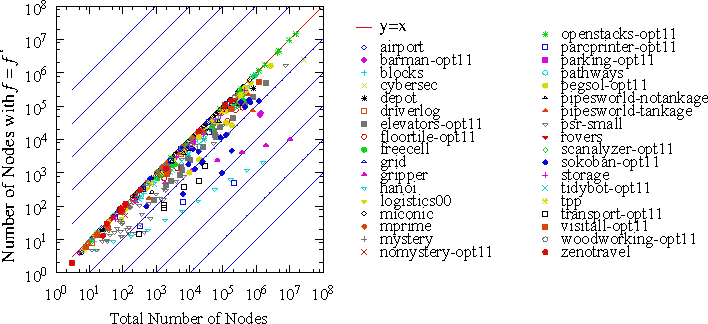
\includegraphics{tables/aaai16-frontier/aaai16prelim3/lmcut_frontier_noh-front.pdf}
 \caption{
 The \# of nodes with $f=f^*$ (y-axis) compared to the
 total \# of nodes in the search space (x-axis) with $f\leq f^*$ on 1104 IPC benchmark problems,
  using modified Fast Downward with \lmcut which 
  generates all nodes with cost $f^*$.
  }
 \label{fig:plateau-noh}
\end{figure}

Therefore, in those majority of IPC problem instances where the size of
the last layer ($f(n)=f^*$) of search is huge, a
\emph{tiebreaking policy} can have a significant impact on the
performance of \astar. Tiebreaking policy is a policy 
for selecting which node to expand among nodes with the same $f$-cost.
It is widely believed that among nodes with the same $f$-cost,
ties should be broken according to $h(n)$, i.e.,
nodes with smaller $h$-values should be expanded first.  While this is a
useful rule of thumb in many domains, it turns out that tiebreaking
requires more careful consideration, particularly for problems with
large \emph{plateaus} -- regions of the search space with the same $f$ and $h$ values.

We first empirically evaluate the existing, commonly used, standard
tiebreaking strategies for \astar.
In the experiments, we show that:
\begin{enumerate}
 \item Last-In-First-Out (\lifo) policy tends to be more efficient
       than a First-In-First-Out (\fifo) policy.
 \item Tiebreaking according to the heuristic value $h$, which
       frequently appears in the heuristic search literature, has little
       impact on the performance as long as a \lifo policy is used.
 \item There are significant performance differences among tiebreaking strategies
       when domains include zero-cost actions.
\end{enumerate}
While there are relatively few domains with zero-cost actions in the
IPC benchmark set, we argue that zero-cost actions naturally occur in 
practical cost-minimization problems.

In order to solve such problems more efficiently, we propose a new
tiebreaking method based on a notion of \emph{depth} within the plateau,
corresponding to the number of steps a node is from the ``entrance'' to
the plateau.  We empirically show that:
\begin{enumerate}
 \item Depth-based diversification strategy significantly outperforms
       other tiebreaking strategies using the same heuristic function.
 \item Artificial gradient introduced by $\epsilon$-cost conversion or
       PLUSONE cost types enforeces the unnecessary best-first expansion order
       within plateau, which essentially makes the task computationally harder.
\end{enumerate}

Note that all tiebreaking strategies in this section maintain the
optimality of the search algorithm because they only affect node
expansion order among the nodes with the same $f$-cost.

\subsubparagraph{gbfs}

After \refsec{sec:gbfs}, we apply the same depth-based diversifying tiebreaking
method to Greedy Best First Search (GBFS) for satisficing planning.

Satisficing search algorithms sacrifices the solution quality for speed,
and GBFS is one extreme of such variants which completely sacrifices the
bounded quality guarantee like those in \astar.  GBFS is heavily used by
various planning solvers in the Satisficing Track of the International
Planning Competition in order to obtain the first solution of a
planning problem.

Dispite the ubiquitous use of GBFS for satisficing search,
various research have suggested that GBFS can be
easily trapped by the undetected dead ends and a huge search plateau.
On infinite graphs, GBFS is not even complete \cite{Valenzano2016}
because it can be misdirected by the heuristic guidance forever.
These pathological behaviors are caused by the fact that 
the search process of GBFS heavily relies upon the
quality of the heuristic function.

The problem is amplified by the fact that GBFS is usually combined
with inadmissible heuristic functions, such as FF
heuristics\cite{Hoffmann01}, Causal Graph heuristics \cite{Helmert2006}, Context Enhanced
Additive (CEA) heuristics\cite{helmert2008unifying}.
% , Landmark-count heuristics\cite{richter2008landmarks}
These functions may overestimate the true distance to the goal,
which can causes some important nodes to be incorrectly labelled as unpromising
(very far from the goal). Best-first search algorithms like GBFS thus
ignores these nodes until after expanding all other nodes with the smaller estimates.

Recently, several approaches
\cite{imai2011novel,valenzano2014comparison,xie14type} have been
proposed for alleviating those problems in GBFS. They improve the search
performance by occasionally ignoring the heuristic guidance, which
provides a chance to recover from the past wrong decisions made by the
heuristics, and makes the algorithm more robust against the heuristic
errors.  These diversified algorithms are probabilistically complete on
the inifinite graphs \cite{Valenzano2016}: The probability of finding a
solution approaches to 1 as the runtime approaches to infinity; in other
words, it eventually finds a solution.

% by relaxing its dependency to the heuristic function.

%% this paragraph is important because diversity, exploration, and
%% ``removing bias'' might not immediately connect with each other
One common theme in these algorithms is to remove the \emph{bias} and
add a \emph{diversity} and \emph{exploration} to the search process.
Exploration, an opposite word to exploitation, is an act of removing
the focus or the bias, thus is equivalent to an act of introducing the
diversity. Hereafter, we use these three key words interchangeably.

In these sections, we show that there is much more room for diversifying
the behavior of GBFS, and show that the use of our depth-based
tiebreaking strategy improves the performance of GBFS by
diversifying the search within the same $h$-plateau.
 
GBFS variants mentioned above all employ the
exploration by occasionally expanding the nodes with bad heuristic
estimates. While this can avoid the problem of large bias of the search
algorithm to the nodes with the least estimates, it cannot detect the bias among the nodes with the same
estimates. Imagine what happens if a heuristic function always returns a
constant value $c$. Since all nodes expanded by GBFS has the same
evaluation $c$, above-mentioned GBFS variants fail to identify their
difference based on the estimates. \footnote{Type-GBFS and DBFS2 can also
diversify the search based on the $g$ value, the current shortest path
cost from the initial state.}

To our knowledge, there are currently no well-established tiebreaking
policy for GBFS.  Compared to \astar, GBFS does not use $f$ and $g$
value during the search process.  The search by GBFS is solely guided by
the heuristic value $h$: It always expands the node with the smallest
$h$ value, and hence the analogy from \astar e.g.\ sorting the nodes
with $f$ and breaking ties according to $h$ is not possible.

% We propose the use of recently proposed tiebreaking strategy based on
% the \emph{depth} of each node from the entrance in the plateau, originally
% designed for \astar, also improves the performance of GBFS by
% diversifying the search within the same h-plateau.
Our depth-based tiebreaking can be implemented as an extension to GBFS, and
can also be incorpolated as a part of type-bucket generation criteria in
Type-Based GBFS.  We empirically evaluate the performance of the
proposed approach, comparing numerous search enhancement techniques such
as Lazy Evaluation, PLUS\-ONE/ONE cost type, Preferred Operators and
Multi-queue heuristic search.

\section{Preliminaries and Definitions}

We first define some notation and terminology used throughout the rest of the paper.
A \emph{tiebreaking strategy} selects from among nodes with the same $f$-value.
Tiebreaking strategies are denoted as $[\text{criterion}_1, \text{criterion}_2, ..., \text{criterion}_k]$,
which means: If there are multiple nodes with the same $f$-value, first, break ties using $\text{criterion}_1$. 
If there are still multiple nodes remaining, then break ties using $\text{criterion}_2$ and so on, until a single node is selected.
The \emph{first-level tiebreaking policy} of a strategy is
$\text{criterion}_1$, the \emph{second-level tiebreaking policy} is
$\text{criterion}_2$, and so on.
%% the word frontier is no longer used in the later text.
% \emph{final frontier} is the set of open nodes with $f^*$.

A \emph{plateau} is a set of nodes in OPEN with both the same $f$ and same $h$ costs.
A plateau whose nodes have $f$-cost $f_p$ and $h$-cost $h_p$ is denoted as
$\plateau{f_p,h_p}$.
An  \emph{entrance} to a $\plateau{f_p,h_p}$ is a node $n \in \plateau{f_p,h_p}$, whose current parent is not a member of $\plateau{f_p,h_p}$.
The \emph{final plateau},  is the plateau containing the solution found by the search algorithm.
In \astar using admissible heuristics, the final plateau is  $\plateau{f^*,0}$.




\section{Background: Tiebreaking Strategies in \astar}

\label{sec:astar-background}


%Aside from the heuristic function, most best-first family of search
%algorithms, including \astar, IDA* and so on, have a tiebreaking criteria which is used
%when two nodes have the same $f$ value.

If multiple nodes with the same $f$-cost are possible, \astar
must implement some tiebreaking policy (either
explicitly or implicitly) which selects from among these nodes.
The early literature on heuristic search seems to have been mostly agnostic regarding tiebreaking.
The original \astar paper, as well as Nilsson's subsequent textbook 
states: ``Select the open node $n$ whose value $f$
is smallest. Resolve ties arbitrarily, but always in favor of any [goal
node]'' \cite[p.102 Step 2]{hart1968formal}, \cite[p.69]{Nilsson71}.
% Although it is possible to interpret this to imply $h$-based tiebreaking
% since goal nodes are the special case where $h=0$,
% they make no further mention of tiebreaking.
Pearl's textbook on heuristic search specifies that best-first search should ``break ties arbitrarily'' (\citeyear{pearl1984heuristics}, p.48, Step 3), and does not specifically mention tiebreaking for \astar.
To the best of our knowledge, the first explicit mention of a tiebreaking policy that considers node generation order is by Korf in his analysis of IDA*: ``If \astar employs the tiebreaking rule of 'most-recently generated', it must also expand the same nodes [as IDA*]'', i.e., a \lifo ordering.

In recent years, tiebreaking according to $h$-values has become ``folklore'' in the search community.
\citeauthor{hansen2007anytime} state that ``It is well-known 
that \astar achieves best performance when it breaks ties
in favor of nodes with least h-cost'' \cite{hansen2007anytime}.
\citeauthor{holte2010common} writes ``\astar breaks ties in favor
of larger $g$-values, as is most often done'' \cite[note that since $f=g+h$,
preferring large $g$ is equivalent to preferring smaller $h$]{holte2010common}.
% \citeauthor{felner2011inconsistent} also assume ``ties are broken in
% favor of low h-values'' in describing Bidirectional Pathmax for \astar.
In their detailed survey/tutorial on efficient \astar implementations,
\citeauthor{burns2012implementing} \citeyear{burns2012implementing}
also break ties ``preferring high $g$'' (equivalent to low $h$).
%% this could be moved to later analysis
% They further write: ``The reasoning is that the goal can be found more
% quickly in the final $f$ layer of search''.
Thus, tiebreaking according to $h$-values appears
to be ubiquitous in practice.
To our knowledge, an in-depth, experimental analysis of tiebreaking strategies for \astar is lacking in the literature.

Although the standard practice of tiebreaking according to $h$ might be
sufficient in some domains, further levels of tiebreaking (explicit or
implicit) are required if multiple nodes can have the same $f$ and
$h$ values.
%% we do, in Roger, Helmert 
% We are not aware of any work that explicitly mentions 2nd-level tiebreaking.
While the survey of efficient \astar implementation techniques in
\cite{burns2012implementing} did not explicitly mention 2nd-level
tiebreaking, their library code ({\footnotesize https://github.com/eaburns/search})
first breaks ties according to $h$, and then
breaks remaining ties according to a \lifo policy (most recently
generated nodes first), i.e., a $[h,\lifo]$ strategy.
Although not documented, their choice of a \lifo 2nd-level tiebreaking policy appears to be a natural consequence of the fact it can be trivially, efficiently implemented in their two-level bucket (vector) implementation of OPEN.
In contrast, the current implementation of the \sota \astar based planner Fast
Downward \cite{Helmert2006}, %\footnote{http://www.fast-downward.org}, <-- takes up 2 lines!
as well as 
the work by \cite{RogerH10} uses a $[h,\fifo]$ tiebreaking strategy.
Although we could not find an explanation, this choice is most likely due to their use of alternating OPEN lists, in which case the \fifo second-level policy serves to provide a limited form of fairness.
%We could not find any explanation for this choice either.


%\citeauthor{Korf1985depth} uses $h$-based tiebreaking in the context of WA*
%\cite{korf1993linear}.  
% ** not sure how/where to put this..

\section{Evaluation of Standard Strategies}
\label{sec:eval-common-strategies}
We evaluated tiebreaking strategies for domain-independent, classical planning.
In our experiments, the planners are based on Fast Downward (revision 6251), and all
experiments are run with a 5-minute, 2GB memory limit for the search binary (FD translation/preprocessing times are not included in the 5-minute limit).
All experiments were conducted on Xeon E5410@2.33GHz CPUs.
We used 1104 instances from 35 standard benchmark domains.
%and 620 problems from 28 \emph{zero-cost-action} domains (\refsec{sec:zerocost-domains}).

\begin{figure*}[htb]
 \newcommand{\minilength}{0.34\textwidth}
 \newcommand{\minisep}{0.02\textwidth}
 \begin{minipage}[t]{\minilength}
  \centering
  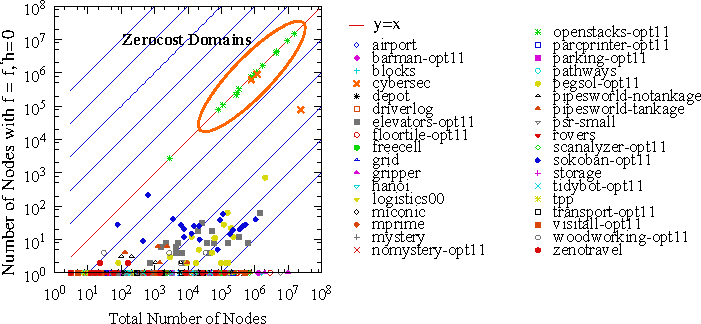
\includegraphics{tables/aaai16-frontier/aaai16prelim3/lmcut_frontier-front.pdf}
  \caption{
  Similar to \refig{fig:plateau-noh}; $y$-axis shows
  \# nodes with $f=f^*, h=0$, which forms the final
  plateau when $h$-based tiebreaking is enabled.
  Note that many \pddl{Openstacks} and \pddl{Cybersec} instances are near the $y=x$ line.
  }
  \label{fig:plateau}
 \end{minipage} 
 \hfill
 \begin{minipage}[t]{0.26\textwidth}
  \centering
  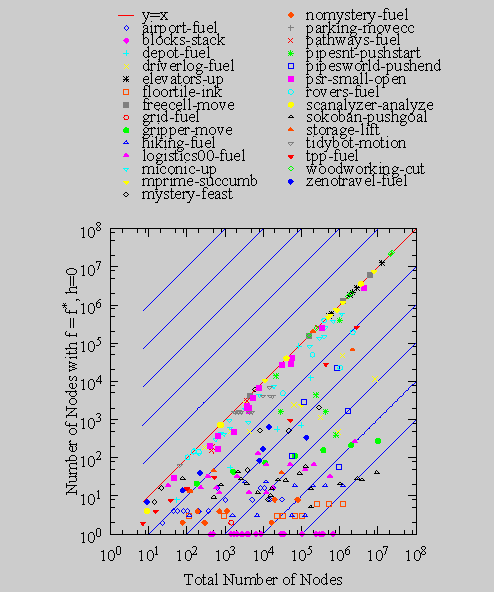
\includegraphics{tables/aaai16-frontier/zerocost/lmcut_frontier-front.pdf}
  \caption{Similar to \refig{fig:plateau}, but for 620 instances from our 
  \emph{zerocost domains} (\refsec{sec:zerocost-domains}),
  where zero-cost actions induce very large plateaus.
 }
 \label{fig:plateau-zerocost}
 \end{minipage}
\end{figure*}


We first compared two commonly used tiebreaking strategies, $[h,\fifo]$, $[h,\lifo]$, which
first break ties according to $h$, and then apply \fifo or \lifo
second-level tiebreaking, respectively.
% The following will be necessary in a future version, if we use LOP:
%Although the search behavior of $[f,h,\fifo]$ corresponds to the default behavior of Fast Downward, this implementation differs 
%from the original, unmodified code because we enabled caching of $h$-values, so that reopened nodes refer to cached $h$-values.\footnote{The current Fast Downward code disables $h$-caching because its current implementation is not compatible with multiple admissible heuristics.}
%Thus, we also show results for unmodified Fast Downward -- as expected, $[f,h,\fifo]$ dominates unmodified FD.
Detailed results for the LMcut heuristic \cite{Helmert2009}, as well as summary results for the M\&S heuristic \cite{HelmertHHN14}, are
shown in \reftbl{tbl:depth} (leftmost 2 columns).
Differences in coverage are observed in several domains, and
$[h,\lifo]$ outperforms $[h,\fifo]$ in total.
\refig{fig:f-h-eval} gives us a
more fine-grained analysis by comparing the number of node evaluation
(computations of \lmcut) of the $[h,\lifo]$ and $[h,\fifo]$ strategies.
It shows that the difference in the \# of nodes
evaluated can sometimes be larger than a factor of 10 (\pddl{Openstacks}, \pddl{Cybersec} domains).
\begin{figure}[tb]
 \centering \relsize{-3}
 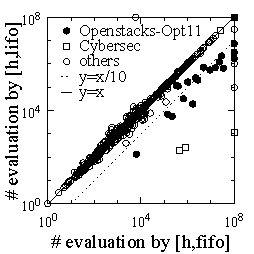
\includegraphics{tables/aaai16-30min-5min-cut/aaai16prelim3/evaluated-lmcut_ff-lmcut_lf-mono.pdf}
 \caption{\# of evaluations of standard \fifo vs
 \lifo second-level tiebreaking, with first-level $h$
 tiebreaking. \lifo evaluates  less than $1/10$ of the nodes evaluated
 by \fifo in \pddl{Cybersec} and \pddl{Openstacks}. 
 }
 \label{fig:f-h-eval}
\end{figure}

\begin{table*}[htb]
 \centering
 \relsize{-1} \setlength{\tabcolsep}{0.3em}
 \begin{tabular}{|c|c|c|c|c|c|c|c|c|c||c|c|c|}
\hline
 & \multicolumn{4}{|c|}{Coverages (\# problems solved)}
 & \multicolumn{5}{|c||}{Coverage (\# problems solved), 10 runs (mean$\pm$sd)}
 & \multicolumn{3}{|c|}{Wilcoxon $p$ vs $[h,\rd,\ro]$} \\
\hline                                    
 Domain &  $[h,\fifo]$ &  $[h,\lifo]$ &  $[\fifo]$ &  $[\lifo]$ &  $[h,\fd,\ro]$ &  $[h,\ld,\ro]$ &  $[h,\rd,\ro]$ &  $[\rd,\ro]$ &  $[h,\ro]$ & $[h,\fd,\ro]$   & $[h,\ld,\ro]$   & $[h,\ro]$    \\
\hline                                    
\lmcut IPC (1104) &  558 &  565 &  442 &  556 &  556.6\spm{}0.7 &  570.3\spm{}2.1 &  \textbf{572.8\spm{}0.7} &  558.8\spm{}2.1 &  559.8\spm{}1.0 &  \textbf{0.0} &  \textbf{.01} &  \textbf{0.0}  \\
\hline                                    
 {\relsize{-1}airport(50)} &  \textbf{27} &  26 &  18 &  26 &  26.2\spm{}0.4 &  26.2\spm{}0.4 &  26.2\spm{}0.4 &  21.0\spm{}0.0 &  26.0\spm{}0.0 &  1.0 &  1.0 &  .17  \\
 {\relsize{-1}barman-opt11(20)} &  0 &  0 &  0 &  0 &  0.0\spm{}0.0 &  0.0\spm{}0.0 &  0.0\spm{}0.0 &  0.0\spm{}0.0 &  0.0\spm{}0.0 &  1.0 &  1.0 &  1.0  \\
 {\relsize{-1}blocks(35)} &  28 &  28 &  26 &  26 &  28.0\spm{}0.0 &  28.0\spm{}0.0 &  28.0\spm{}0.0 &  26.9\spm{}0.5 &  28.0\spm{}0.0 &  1.0 &  1.0 &  1.0  \\
 {\relsize{-1}cybersec(19)} &  2 &  3 &  0 &  3 &  2.0\spm{}0.0 &  8.5\spm{}2.0 &  \textbf{10.9\spm{}0.8} &  7.4\spm{}0.7 &  4.4\spm{}1.0 &  \textbf{0.0} &  \textbf{.01} &  \textbf{0.0}  \\
 {\relsize{-1}depot(22)} &  6 &  6 &  5 &  5 &  6.0\spm{}0.0 &  6.0\spm{}0.0 &  6.0\spm{}0.0 &  6.0\spm{}0.0 &  6.0\spm{}0.0 &  1.0 &  1.0 &  1.0  \\
 {\relsize{-1}driverlog(20)} &  13 &  13 &  12 &  13 &  13.0\spm{}0.0 &  13.0\spm{}0.0 &  13.0\spm{}0.0 &  12.9\spm{}0.3 &  13.0\spm{}0.0 &  1.0 &  1.0 &  1.0  \\
 {\relsize{-1}elevators-opt11(20)} &  15 &  15 &  14 &  15 &  15.0\spm{}0.0 &  15.0\spm{}0.0 &  15.0\spm{}0.0 &  14.6\spm{}0.5 &  15.0\spm{}0.0 &  1.0 &  1.0 &  1.0  \\
 {\relsize{-1}floortile-opt11(20)} &  6 &  6 &  6 &  6 &  6.0\spm{}0.0 &  6.0\spm{}0.0 &  6.0\spm{}0.0 &  6.0\spm{}0.0 &  6.0\spm{}0.0 &  1.0 &  1.0 &  1.0  \\
 {\relsize{-1}freecell(80)} &  9 &  9 &  8 &  9 &  9.0\spm{}0.0 &  9.0\spm{}0.0 &  9.0\spm{}0.0 &  9.0\spm{}0.0 &  9.0\spm{}0.0 &  1.0 &  1.0 &  1.0  \\
 {\relsize{-1}grid(5)} &  1 &  1 &  1 &  1 &  1.0\spm{}0.0 &  1.0\spm{}0.0 &  1.0\spm{}0.0 &  1.0\spm{}0.0 &  1.0\spm{}0.0 &  1.0 &  1.0 &  1.0  \\
 {\relsize{-1}gripper(20)} &  6 &  6 &  6 &  6 &  6.0\spm{}0.0 &  6.0\spm{}0.0 &  6.0\spm{}0.0 &  6.0\spm{}0.0 &  6.0\spm{}0.0 &  1.0 &  1.0 &  1.0  \\
 {\relsize{-1}hanoi(30)} &  12 &  12 &  12 &  12 &  12.0\spm{}0.0 &  12.0\spm{}0.0 &  12.0\spm{}0.0 &  12.0\spm{}0.0 &  12.0\spm{}0.0 &  1.0 &  1.0 &  1.0  \\
 {\relsize{-1}logistics00(28)} &  \textbf{20} &  \textbf{20} &  16 &  18 &  \textbf{20.0\spm{}0.0} &  \textbf{20.0\spm{}0.0} &  \textbf{20.0\spm{}0.0} &  \textbf{20.0\spm{}0.0} &  \textbf{20.0\spm{}0.0} &  1.0 &  1.0 &  1.0  \\
 {\relsize{-1}miconic(150)} &  \textbf{140} &  \textbf{140} &  68 &  \textbf{140} &  \textbf{140.0\spm{}0.0} &  \textbf{140.0\spm{}0.0} &  \textbf{140.0\spm{}0.0} &  135.5\spm{}1.2 &  \textbf{140.0\spm{}0.0} &  1.0 &  1.0 &  1.0  \\
 {\relsize{-1}mprime(35)} &  21 &  21 &  19 &  22 &  21.0\spm{}0.0 &  21.0\spm{}0.0 &  21.0\spm{}0.0 &  21.0\spm{}0.0 &  20.9\spm{}0.3 &  1.0 &  1.0 &  .37  \\
 {\relsize{-1}mystery(30)} &  15 &  16 &  15 &  15 &  15.0\spm{}0.0 &  15.0\spm{}0.0 &  15.0\spm{}0.0 &  15.5\spm{}0.5 &  15.0\spm{}0.0 &  1.0 &  1.0 &  1.0  \\
 {\relsize{-1}nomystery-opt11(20)} &  14 &  14 &  12 &  13 &  14.0\spm{}0.0 &  14.0\spm{}0.0 &  14.0\spm{}0.0 &  13.7\spm{}0.5 &  14.0\spm{}0.0 &  1.0 &  1.0 &  1.0  \\
 {\relsize{-1}openstacks-opt11(20)} &  11 &  \textbf{18} &  11 & \textbf{18} &  11.0\spm{}0.0 &  \textbf{18.0\spm{}0.0} & \textbf{18.0\spm{}0.0} &  \textbf{18.0\spm{}0.0} &  11.6\spm{}0.5 &  \textbf{0.0} &  1.0 &  \textbf{0.0}  \\
 {\relsize{-1}parcprinter-opt11(20)} &  13 &  13 &  12 &  13 &  13.0\spm{}0.0 &  13.0\spm{}0.0 &  13.0\spm{}0.0 &  13.0\spm{}0.0 &  13.0\spm{}0.0 &  1.0 &  1.0 &  1.0  \\
 {\relsize{-1}parking-opt11(20)} &  1 &  1 &  1 &  1 &  1.0\spm{}0.0 &  1.0\spm{}0.0 &  1.0\spm{}0.0 &  1.0\spm{}0.0 &  1.0\spm{}0.0 &  1.0 &  1.0 &  1.0  \\
 {\relsize{-1}pathways(30)} &  5 &  5 &  4 &  5 &  5.0\spm{}0.0 &  5.0\spm{}0.0 &  5.0\spm{}0.0 &  5.0\spm{}0.0 &  5.0\spm{}0.0 &  1.0 &  1.0 &  1.0  \\
 {\relsize{-1}pegsol-opt11(20)} &  17 &  17 &  17 &  17 &  17.0\spm{}0.0 &  17.0\spm{}0.0 &  17.0\spm{}0.0 &  17.0\spm{}0.0 &  17.0\spm{}0.0 &  1.0 &  1.0 &  1.0  \\
 {\relsize{-1}pipesworld-notankage(50)} &  \textbf{15} &  14 &  13 &  13 &  14.4\spm{}0.5 &  14.6\spm{}0.5 &  14.7\spm{}0.5 &  14.3\spm{}0.5 &  14.9\spm{}0.3 &  0.2 &  .68 &  0.3  \\
 {\relsize{-1}pipesworld-tankage(50)} &  8 &  8 &  7 &  8 &  8.0\spm{}0.0 &  8.0\spm{}0.0 &  8.0\spm{}0.0 &  8.0\spm{}0.0 &  8.0\spm{}0.0 &  1.0 &  1.0 &  1.0  \\
 {\relsize{-1}psr-small(50)} &  48 &  48 &  48 &  48 &  48.0\spm{}0.0 &  48.0\spm{}0.0 &  48.0\spm{}0.0 &  48.0\spm{}0.0 &  48.0\spm{}0.0 &  1.0 &  1.0 &  1.0  \\
 {\relsize{-1}rovers(40)} &  7 &  7 &  7 &  7 &  7.0\spm{}0.0 &  7.0\spm{}0.0 &  7.0\spm{}0.0 &  7.0\spm{}0.0 &  7.0\spm{}0.0 &  1.0 &  1.0 &  1.0  \\
 {\relsize{-1}scanalyzer-opt11(20)} &  \textbf{10} &  \textbf{10} &  4 &  \textbf{10} &  \textbf{10.0\spm{}0.0} &  \textbf{10.0\spm{}0.0} &  \textbf{10.0\spm{}0.0} &  9.0\spm{}0.0 &  \textbf{10.0\spm{}0.0} &  1.0 &  1.0 &  1.0  \\
 {\relsize{-1}sokoban-opt11(20)} &  19 &  19 &  19 &  19 &  19.0\spm{}0.0 &  19.0\spm{}0.0 &  19.0\spm{}0.0 &  19.0\spm{}0.0 &  19.0\spm{}0.0 &  1.0 &  1.0 &  1.0  \\
 {\relsize{-1}storage(30)} &  14 &  14 &  14 &  14 &  14.0\spm{}0.0 &  14.0\spm{}0.0 &  14.0\spm{}0.0 &  14.5\spm{}0.5 &  14.0\spm{}0.0 &  1.0 &  1.0 &  1.0  \\
 {\relsize{-1}tidybot-opt11(20)} &  12 &  12 &  11 &  11 &  12.0\spm{}0.0 &  12.0\spm{}0.0 &  12.0\spm{}0.0 &  11.9\spm{}0.3 &  12.0\spm{}0.0 &  1.0 &  1.0 &  1.0  \\
 {\relsize{-1}tpp(30)} &  6 &  6 &  6 &  6 &  6.0\spm{}0.0 &  6.0\spm{}0.0 &  6.0\spm{}0.0 &  6.0\spm{}0.0 &  6.0\spm{}0.0 &  1.0 &  1.0 &  1.0  \\
 {\relsize{-1}transport-opt11(20)} &  6 &  6 &  6 &  6 &  6.0\spm{}0.0 &  6.0\spm{}0.0 &  6.0\spm{}0.0 &  6.0\spm{}0.0 &  6.0\spm{}0.0 &  1.0 &  1.0 &  1.0  \\
 {\relsize{-1}visitall-opt11(20)} &  10 &  10 &  9 &  10 &  10.0\spm{}0.0 &  10.0\spm{}0.0 &  10.0\spm{}0.0 &  10.0\spm{}0.0 &  10.0\spm{}0.0 &  1.0 &  1.0 &  1.0  \\
 {\relsize{-1}woodworking-opt11(20)} &  10 &  10 &  6 &  9 &  10.0\spm{}0.0 &  10.0\spm{}0.0 &  10.0\spm{}0.0 &  \textbf{11.6\spm{}0.5} &  10.0\spm{}0.0 &  1.0 &  1.0 &  1.0  \\
 {\relsize{-1}zenotravel(20)} &  11 &  11 &  9 &  11 &  11.0\spm{}0.0 &  11.0\spm{}0.0 &  11.0\spm{}0.0 &  11.0\spm{}0.0 &  11.0\spm{}0.0 &  1.0 &  1.0 &  1.0 \\
\hline
\lmcut Zerocost(620) &  256 &  279 &  212 &  281 &  257.4\spm{}2.0 &  286.6\spm{}7.1 &  \textbf{294.2\spm{}2.3} &  279.9\spm{}3.9 &  264.9\spm{}1.8 &  \textbf{0.0} &  \textbf{.01} &  \textbf{0.0}  \\
\hline                                    
 {\relsize{-1}airport-fuel(20)} &  \textbf{15} &  13 &  7 &  \textbf{15} &  14.7\spm{}1.0 &  14.0\spm{}0.6 &  14.6\spm{}0.5 &  10.5\spm{}0.7 &  14.4\spm{}0.7 &  .59 &  \textbf{.05} &  .58  \\
 {\relsize{-1}blocks-stack(20)} &  17 &  17 &  15 &  17 &  17.0\spm{}0.0 &  17.1\spm{}0.3 &  17.2\spm{}0.4 &  16.3\spm{}0.5 &  17.0\spm{}0.0 &  .17 &  .58 &  .17  \\
 {\relsize{-1}depot-fuel(22)} &  6 &  6 &  4 &  6 &  6.0\spm{}0.0 &  6.0\spm{}0.0 &  6.0\spm{}0.0 &  6.0\spm{}0.0 &  6.0\spm{}0.0 &  1.0 &  1.0 &  1.0  \\
 {\relsize{-1}driverlog-fuel(20)} &  \textbf{8} &  \textbf{8} &  7 &  \textbf{8} & \textbf{ 8.0\spm{}0.0} &  7.7\spm{}0.5 &  \textbf{8.0\spm{}0.0} &  \textbf{8.0\spm{}0.0} &  \textbf{8.0\spm{}0.0} &  1.0 &  .08 &  1.0  \\
 {\relsize{-1}elevators-up(20)} &  7 &  \textbf{13} &  7 &  \textbf{13} &  7.0\spm{}0.0 &  9.4\spm{}0.7 &  10.7\spm{}1.1 &  8.3\spm{}0.6 &  7.3\spm{}0.5 &  \textbf{0.0} &  \textbf{.02} &  \textbf{0.0}  \\
 {\relsize{-1}floortile-ink(20)} &  8 &  8 &  8 &  8 &  8.0\spm{}0.0 &  8.0\spm{}0.0 &  8.1\spm{}0.3 &  8.1\spm{}0.3 &  8.3\spm{}0.5 &  .37 &  .37 &  0.3  \\
 {\relsize{-1}freecell-move(20)} &  4 &  19 &  4 & 19 &  4.0\spm{}0.0 &  \textbf{19.7\spm{}0.5} &  17.2\spm{}0.6 &  16.7\spm{}1.0 &  5.0\spm{}0.4 &  \textbf{0.0} &  \textbf{0.0} &  \textbf{0.0}  \\
 {\relsize{-1}grid-fuel(5)} &  1 &  1 &  1 &  1 &  1.0\spm{}0.0 &  1.0\spm{}0.0 &  1.0\spm{}0.0 &  1.0\spm{}0.0 &  1.0\spm{}0.0 &  1.0 &  1.0 &  1.0  \\
 {\relsize{-1}gripper-move(20)} &  7 &  7 &  7 &  7 &  7.0\spm{}0.0 &  7.0\spm{}0.0 &  7.0\spm{}0.0 &  7.0\spm{}0.0 &  7.0\spm{}0.0 &  1.0 &  1.0 &  1.0  \\
 {\relsize{-1}hiking-fuel(20)} &  9 &  9 &  8 &  9 &  9.0\spm{}0.0 &  9.0\spm{}0.0 &  9.0\spm{}0.0 &  9.0\spm{}0.0 &  9.0\spm{}0.0 &  1.0 &  1.0 &  1.0  \\
 {\relsize{-1}logistics00-fuel(28)} &  16 &  16 &  15 &  16 &  16.0\spm{}0.0 &  16.0\spm{}0.0 &  16.0\spm{}0.0 &  16.0\spm{}0.0 &  16.0\spm{}0.0 &  1.0 &  1.0 &  1.0  \\
 {\relsize{-1}miconic-up(30)} &  16 &  17 &  10 &  17 &  15.7\spm{}0.5 &  19.4\spm{}0.7 &  \textbf{20.4\spm{}1.2} &  \textbf{20.4\spm{}0.9} &  17.0\spm{}0.4 &  \textbf{0.0} &  \textbf{.03} &  \textbf{0.0}  \\
 {\relsize{-1}mprime-succumb(35)} &  15 &  14 &  12 &  14 &  16.3\spm{}0.5 &  18.9\spm{}4.0 &  \textbf{20.5\spm{}0.8} &  18.1\spm{}1.6 &  17.9\spm{}0.5 &  \textbf{0.0} &  .15 &  \textbf{0.0}  \\
 {\relsize{-1}mystery-feast(20)} &  7 &  5 &  5 &  5 &  7.4\spm{}0.5 &  6.7\spm{}0.8 &  7.5\spm{}0.5 &  6.9\spm{}0.7 &  7.3\spm{}0.5 &  .69 &  \textbf{.03} &  0.4  \\
 {\relsize{-1}nomystery-fuel(20)} &  10 &  10 &  9 &  10 &  10.0\spm{}0.0 &  10.0\spm{}0.0 &  10.0\spm{}0.0 &  9.5\spm{}0.5 &  10.0\spm{}0.0 &  1.0 &  1.0 &  1.0  \\
 {\relsize{-1}parking-movecc(20)} &  0 &  0 &  0 &  0 &  0.0\spm{}0.0 &  0.0\spm{}0.0 &  0.0\spm{}0.0 &  0.0\spm{}0.0 &  0.0\spm{}0.0 &  1.0 &  1.0 &  1.0  \\
 {\relsize{-1}pathways-fuel(30)} &  5 &  5 &  4 &  5 &  5.0\spm{}0.0 &  4.2\spm{}0.4 &  4.5\spm{}0.5 &  4.9\spm{}0.3 &  4.4\spm{}0.5 &  \textbf{.01} &  .19 &  .69  \\
 {\relsize{-1}pipesnt-pushstart(20)} &  8 &  8 &  6 &  7 &  8.0\spm{}0.0 &  8.8\spm{}1.3 &  \textbf{9.8\spm{}0.4} &  9.7\spm{}0.5 &  8.5\spm{}0.5 &  \textbf{0.0} &  0.1 &  \textbf{0.0}  \\
 {\relsize{-1}pipesworld-pushend(20)} &  3 &  4 &  2 &  4 &  3.0\spm{}0.0 &  4.2\spm{}1.0 &  4.9\spm{}0.5 &  \textbf{5.2\spm{}1.2} &  3.9\spm{}0.3 &  \textbf{0.0} &  .09 &  \textbf{0.0}  \\
 {\relsize{-1}psr-small-open(20)} &  19 &  19 &  19 &  19 &  19.0\spm{}0.0 &  19.0\spm{}0.0 &  19.0\spm{}0.0 &  19.0\spm{}0.0 &  19.0\spm{}0.0 &  1.0 &  1.0 &  1.0  \\
 {\relsize{-1}rovers-fuel(40)} &  8 &  8 &  7 &  9 &  8.0\spm{}0.0 &  8.0\spm{}0.0 &  8.0\spm{}0.0 &  9.0\spm{}0.0 &  8.0\spm{}0.0 &  1.0 &  1.0 &  1.0  \\
 {\relsize{-1}scanalyzer-analyze(20)} &  9 &  9 &  3 &  9 &  \textbf{9.8\spm{}0.9} &  9.4\spm{}0.5 &  9.2\spm{}0.4 &  7.3\spm{}1.0 &  9.1\spm{}0.3 &  .07 &  .37 &  .58  \\
 {\relsize{-1}sokoban-pushgoal(20)} &  18 &  18 &  18 &  18 &  18.0\spm{}0.0 &  17.0\spm{}0.0 &  18.0\spm{}0.0 &  17.0\spm{}0.0 &  18.0\spm{}0.0 &  1.0 &  \textbf{0.0} &  1.0  \\
 {\relsize{-1}storage-lift(20)} &  4 &  4 &  4 &  4 &  4.0\spm{}0.0 &  5.2\spm{}1.2 &  4.4\spm{}0.5 &  4.6\spm{}0.5 &  4.6\spm{}0.5 &  \textbf{.03} &  .12 &  .41  \\
 {\relsize{-1}tidybot-motion(20)} &  16 &  16 &  14 &  16 &  16.0\spm{}0.0 &  16.0\spm{}0.0 &  16.0\spm{}0.0 &  15.7\spm{}0.5 &  16.0\spm{}0.0 &  1.0 &  1.0 &  1.0  \\
 {\relsize{-1}tpp-fuel(30)} &  8 &  \textbf{11} &  7 &  \textbf{11} &  7.5\spm{}0.5 &  \textbf{11.0\spm{}0.0} &  \textbf{11.0\spm{}0.0} &  \textbf{11.0\spm{}0.0} &  8.1\spm{}0.3 &  \textbf{0.0} &  1.0 &  \textbf{0.0}  \\
 {\relsize{-1}woodworking-cut(20)} &  5 &  7 &  2 &  7 &  5.0\spm{}0.0 &  6.9\spm{}0.3 &  \textbf{9.2\spm{}0.9} &  7.7\spm{}0.6 &  7.1\spm{}0.3 &  \textbf{0.0} &  \textbf{0.0} &  \textbf{0.0}  \\
 {\relsize{-1}zenotravel-fuel(20)} &  7 &  7 &  7 &  7 &  7.0\spm{}0.0 &  7.0\spm{}0.0 &  7.0\spm{}0.0 &  7.0\spm{}0.0 &  7.0\spm{}0.0 &  1.0 &  1.0 &  1.0 \\
\hline
\lmcut Total(1724) &  814 &  844 &  654 &  837 &  814.0\spm{}2.3 &  856.9\spm{}8.5 &  \textbf{867.0\spm{}2.1} &  838.7\spm{}4.9 &  824.7\spm{}2.1 &  \textbf{0.0} &  \textbf{.01} &  \textbf{0.0} \\
\hline
\hline
\mands IPC (1104) &  479 &  \textbf{488} &  451 &  481 &  478.8\spm{}0.4 &  484.8\spm{}0.4 &  484.0\spm{}0.0 &  481.4\spm{}1.4 &  486.4\spm{}0.8 &  \textbf{.01} &  \textbf{.02} &  \textbf{.01}  \\
\mands Zerocost (620) &  276 &  290 &  226 &  283 &  274.0\spm{}0.9 &  293.4\spm{}2.1 &  \textbf{310.2\spm{}2.1} &  303.2\spm{}1.7 &  288.0\spm{}1.7 &  \textbf{.01} &  \textbf{.01} &  \textbf{.01}  \\
\mands Total(1724) &  755 &  778 &  677 &  764 &  752.8\spm{}0.7 &  778.2\spm{}1.9 &  \textbf{794.2\spm{}2.1} &  784.6\spm{}2.1 &  774.4\spm{}1.2 &  \textbf{.01} &  \textbf{.01} &  \textbf{.01} \\
\hline
\end{tabular}

 \caption{Coverage comparison (\# of instances solved in 5min, 2GB), \textbf{bold}=best. Zerocost domains are named as [original name]-[name of nonzero action]. Due to space, we only show the domains whose maximum pairwise coverage difference $\mit{MaxDiff}>2$. (We used the means of 10 runs for the randomized strategies.) Domains with $\mit{MaxDiff}\leq 2$ follows:
 (1) $\mit{MaxDiff} = 0$ (same coverages by all configuration and all runs): \pddls{barman-opt11, floortile-opt11, grid, gripper, hanoi, parking-opt11, pegsol-opt11, psr-small, rovers, sokoban-opt11, tpp, transport-opt11, grid-fuel, gripper-move, parking-movecc, psr-small-open, zenotravel-fuel}.
 (2) $0 < \mit{MaxDiff} \leq 1$: \pddls{depot, driverlog, elevators-opt11, freecell, mystery, parcprinter-opt11, pathways, pipesworld-tankage, storage, tidybot-opt11, visitall-opt11, driverlog-fuel, floortile-ink, hiking-fuel, logistic00-fuel, nomystery-fuel, pathways-fuel, sokoban-pushgoal}.
 (3) $1 < \mit{MaxDiff} \leq 2$: \pddls{blocks, nomystery-opt11, pipesworld-notankage, zenotravel, depot-fuel, rovers-fuel, storage-lift, tidybot-motion}.
 }\label{tbl:depth}
\end{table*}

\subsubsection{Is $h$-Based Tiebreaking Necessary?}
\label{sec:h-necessary}
%Next, we investigated whether $h$-based, first-level tiebreaking is necessary.
\reftbl{tbl:depth} also shows the results of $[\fifo]$ and $[\lifo]$,
which rely only on \fifo or \lifo tiebreaking.
$[\lifo]$, which simply breaks ties among nodes with the same $f$-cost by expanding most recently generated nodes first \cite{korf1985depth}, clearly dominates $[\fifo]$.

Interestingly, the performance of the $[\lifo]$ strategy
is comparable to $[h,\lifo]$ and $[h,\fifo]$, the standard two-level strategies that first break ties according to $h$.
This may be surprising, considering the ubiquity of $h$-based tiebreaking in the search and planning communities.
% 
However, \lifo behaves somewhat similarly to $h$-based tiebreaking, in the following sense:
\lifo expands the most recently generated node $n$.
For any child $n'$, 
if the heuristic function is admissible and $f(n') = f(n)$, there are only 2 possibilities :
(1) $g(n') > g(n)$ and $h(n') < h(n)$, or
(2) $g(n') = g(n)$ and $h(n') = h(n)$,
because $g(n)+h(n)=g(n')+h(n')$.
Thus, as \lifo expands nodes in a ``depth-first'' manner,
the nodes that continue to be expanded by \lifo's depth-first
exploration have non-increasing $h$-values, much like in $h$-based tiebreaking.
Although in general, the expansion order of $[\lifo]$ is not the same 
as that of $h$-based tiebreaking strategies,
this might explain why their performances are comparable.
An in-depth investigation of the behavior of $[\lifo]$ vs. $h$-based tiebreaking is a direction for future work.

% Compared to the $h$-based variants which explicitly selects nodes with smaller $h$ and its expanded nodes have non-increasing $h$-values,
% This has the same  can behave somewhat similarly to actively expanding nodes with low $h$-values, as done by $h$-based tiebreaking.

% \citeauthor{burns2012implementing}
% (\citeyear{burns2012implementing}) writes ``the goal can be found more
% quickly in the final $f$ layer of search'' about $h$ tiebreaking.

\subsubsection{Plateaus and Tiebreaking}

In \refig{fig:f-h-eval},
we observed that large performance differences between
2-level tiebreaking strategies $[h,\lifo]$ and $[h,\fifo]$ tend
to occur in problems where there are many nodes with the same $f$ and
$h$ values, creating large plateau regions where the heuristic does not
provide any useful guidance -- by definition, these plateau regions 
require a blind search (because all nodes
have the same $f,h$) which relies solely on the tiebreaking criterion.

\refig{fig:plateau} plots the size of the final plateau on 1104 IPC
benchmark instances.
The $y$-axis
represents the \# of nodes with $f=f^*, h=0$, i.e., the final plateau, and the $x$-axis represents the total
\# of nodes with $f\leq f^*$.
In some domains such as \pddl{Openstacks} and \pddl{Cybersec}, the planner spends most of the runtime
searching the final plateau even with $h$ tiebreaking, and
thus the runtime on these domains varies significantly depending on the second-level tiebreaking strategy.

\section{Domains with Zero-Cost Actions}
\label{sec:zerocost-domains}
%% best to put openstacks here, considering the connection to the
%% previous section
\pddl{Openstacks}  is a cost
minimization domain introduced in IPC-2006, where the objective is to 
minimize the number of stacks used.
There are many zero-cost actions (i.e., actions that don't increase the number of stacks), and
they prevent the standard heuristics from producing
informative guidance.

%% safe to remove these explanation.
% According to \cite{richter2010lama}, \textbf{??????}
% %Richter talks about the failures on openstacks starting around p.167
% \lmcut \cite{Helmert2009} fails to find a good cost
% partitioning with non-zero values, 
% % A detailed discussion of Openstacks domain and poor performance of landmarks is in \cite{richter10lama}, p.167-169.
% and most edges in the abstraction
% space of M\&S \cite{helmert2007flexible} have zero costs.


% XXX I'm commenting out the paragraphs below because:
% (1) A review of heuristic functions for domain-independent learning is not really
% necessary for this AAAI submission. 
% (2) It's better if this paper is not so strongly associated with the ICAPS community only -- this work applies in general to search with A*, and is not strongly tied to almost-perfect heuristics, lmcut, m&s, etc.

Although domains with zero-cost actions are not common in the current set of benchmarks, we argue that such domains are of an important class of models for cost-minimization problems, i.e.,
assigning zero costs make sense from a practical, modeling perspective.
For example, consider the \pddl{driverlog} domain, where the task is to move packages between locations using trucks.
The IPC version of this domain assigns unit costs to all actions. Thus, cost-optimal planning on this domain seeks to minimize the number of steps in the plan.
However, another natural objective function would be the one which minimizes the amount of fuel spent by driving the trucks,
assigning cost 0 to all actions except \pddl{drive-truck}.

% While I agree with the point you're trying to make,
% There is an ugly issue when arguing that current models try to  optimize plan-execution time (i.e., makespan), 
% which is that if we really cared about makespan optimality, we would consider parallel execution of actions whenever possible.
% however, sequential classical planners do not handle parallel actions at all  (recall ACP).
% so arguing this path can only lead to trouble.. Let's try a safer line of argument.
%% For runtime minimization,
%% nonzero positive costs are reasonable because
%% every actions are supposed to consume a fraction of time.
%% However, such formulation is not suitable for general optimization
%% problems.  For example, when you try to minimize the energy consumption
%% by the elevators in \pddl{Elevators} domain, many actions would have zero-cost
%% --- it does not consume electricity for either boarding or leaving the
%% passenger, or moving the elevator down.
%% % 
%% From the practical point of
%% view, cost minimization domains would have wider interest compared to
%% the simple runtime minimization.
%% Also, as shown previously, such domains pose a
%% difficulty to the current heuristic planners due to their large plateaus.

Similarly, for many practical applications, a natural 
objective is to optimize the usage of one key consumable resource, e.g., fuel/energy minimization.
In fact, two of the IPC domains, \pddl{Openstacks} and \pddl{Cybersec}, which were shown difficult for standard tiebreaking methods in the previous section, both contain many zero-cost actions, and both are based on industrial applications:  \pddl{Openstacks} models production planning \cite{fink1999applications} and \pddl{Cybersec} models Behavioral Adversary Modeling System \cite[minimizing decryption, data transfer, etc.]{boddy2005course}.

Therefore, in this paper, we modified various domains
into cost minimization domains with many zero-cost actions.
Specifically, the domain is modified so that all action schemas are assigned
cost 0 except for 1 action schema which consumes some key resource.
The last word in the names of these domains indicate the action which is assigned non-zero cost, e.g., \pddl{elevator-up} is a modified elevator domain where the \pddl{up} action is assigned non-zero cost, and all other actions have 0 cost.
Most of the transportation-type domains are modified to optimize 
energy usage (\pddl{Logistics-fuel}, \pddl{elevator-up} etc.), and  assembly-type domains are modified to minimize resource usage
%% floortile-ink is not shown, so better not to mention it
(\pddl{Woodworking-cut} minimizes wood usage, etc.).
We did not
include domains with only a single action schema and standard domains which already had many
zero-cost actions (these are already in the results for standard IPC domains).
We refer to these 28 new domains as \emph{zerocost domains}.

\refig{fig:plateau-zerocost} plots the size of the final plateau of the zerocost domain instances.
As expected, many of these zerocost domains have large plateaus.
Thus, in these cost-minimization problems, the search strategy within
plateaus, i.e., tiebreaking,  becomes very important.


\section{Depth-Based Tiebreaking for A*}

\label{sec:depth}

In order to solve zerocost problems, the planner needs to perform an
efficient knowledge-free search within a large, final plateau.
One useful notion which can be used to both understand and control the
search in this situation is the \emph{depth} of a node, which represents
the number of steps (edges in the search space graph) from the entrance of the plateau.  Given a node $n$,
if its current parent $\parent{n}$ is from the other plateau, i.e.,
$\parent{n}$ has a different $f$-value, or different $h$-value when the
first tiebreaking is present, then $\depth{n} = 0$. Nodes with
$\depth{n} = 0$ correspond to the \emph{entrance} of the plateau.  If $n$
and $\parent{n}$ are in the same plateau i.e.\ share the same $f$ and $h$,
$\depth{n}$ is defined as $\depth{\parent{n}} + 1$.  Based on this
simple notion of depth, we propose three \emph{depth-based
tiebreaking} strategies, where the nodes are inserted into buckets associated with
depths, and upon expansion, the buckets are chosen according to some policy.
``First depth'' (\fd), ``last depth'' (\ld), and ``random depth'' (\rd) 
choose a bucket with the smallest depth,
the largest depth, and a depth randomly selected at each expansion, respectively.

\todo{remove this part if complete plot in \refig{fig:depth-histogram} did
not succeed}
The effectiveness of each of these depth-based policies depends on the
problem instance.  Within
the plateau region, all nodes have the same $f$ and $h$ values, 
% yes, for simplicity, I'm assuming 3-level tiebreaks, ignoring no-h for the time being..
and the goals can be near or far
from the entrance.  In the former case, the
search should be focused around the entrance favoring the smaller depths
(\fd), and the behavior in the plateau should be much like breadth-first. In the
latter case, the planner should greedily explore the various area of the
plateau by preferring largest depth (\ld), much like in
depth-first. 
It may also be possible for a goal to be at an intermediate depth, in which case
\fd could take too much time to reach that
depth, and \ld may greedily pass and miss that depth.
By an adversary argument, \rd, which selects a random depth and has no depth bias would seem to be the safest policy.

Depth-based tiebreaking has no effect when used as a second-level tirebreaking policy with a domain with positive costs only \emph{and} $h$-based first-level tiebreaking policy. This is because most actions result in an updated $h$-value, so almost all nodes have depth 0.
% (with consistent heuristics, \emph{all} actions update $h$ and no nodes have depth $\geq 1$)

\subsubsection{Tiebreaking within Depth Buckets}
% changing from ``third-level'' because we'll also consider that sue depth as the 1st-level policy, e.g., [rd,random] (noh).
Since there can be multiple nodes within the same depth bucket,
a further tiebreaking criterion may be necessary to break ties among them.
We could, for example, apply \lifo or \fifo policies at this level -- 
note that $[h,\fd,\fifo]$ and $[h,\ld,\lifo]$ are equivalent to $[h,\fifo]$ and $[h,\lifo]$, respectively.

However we use a Random Order (\ro) policy, which 
randomly selects an element from the depth bucket selected by the depth-based tiebreaking.
This is because the effectiveness of the tiebreaking behavior within a bucket
can be affected by accidental biases, e.g., names/orders of action schema in the PDDL domain
definition \cite{vallati2015effective}.
%Finding the best action ordering is not the scope of this paper.
Thus, we avoid bias at this level of tiebreaking by using \ro and assess its expected/average
performance.



% Among \fifo, \lifo and \ro, the natural policy is Random Order.
% This is because the effectiveness of the third-level tiebreaking behavior
% is affected by the accidental bias in action ordering in the PDDL domain
% definition.  Recent work \cite{vallati2015effective} showed that the
% planner performance is greatly affected by changing and tuning the action ordering
% (and also variable ordering, but it is irrelevant to the tiebreaking behavior). 
% However, finding the best third-level tiebreaking is not the scope of this paper.
% Thus, focusing on \ro and assess its expected/average
% performance is the most reasonable practice to understand the behavior of second-level,
% depth-based tiebreaking.


\subsection{Evaluating Depth-Based Tiebreaking}
\label{sec:depth-based-evaluation}
We evaluated three 3-level tiebreaking strategies.
%% may not be necessary, since they are straw-mans
% and four 2-level tiebreaking strategies in all.
%REDUNDANT? , i.e., $[f,h,depthStrategy,LFR]$, where the first-level tiebreaking is according to $h$ (break ties in favor of small $h$), the second-level strategy is based on depth and $depthStrategy \in \{\fd, \ld, \rd\}$, and the third level tiebreaking strategy $LFR \in \{\lifo, \fifo, \ro\}$.
% 
In addition to the 35 IPC benchmark domains with 1104 instances used in
the previous set of experiments, we used 28 zerocost domains with 620
instances. For randomized strategies, we
show the coverage (mean $\pm$ sd) on
10 independent runs.

% This comparison below may be useful in a future version of the paper, but not necessary in this version.
%% First, we compared $[h,\ld,\lifo]$ and $[h,\fd,\fifo]$
%% with $[h,\lifo]$ and $[h,\fifo]$, respectively, in order to see
%% the extra cost of managing the depth-based buckets.
%% The node evaluation order of $[h,\fd,\fifo]$ and $[h,\ld,\lifo]$
%% are exactly the same as $[h,\fifo]$ and $[h,\lifo]$.
%% This is because:
%% (1) $[h,\lifo]$ expands the most recently evaluated/inserted
%% states, and (2) the depth increases monotonically within the same $[f,h]$,
%% thus (3) $[h,\lifo]$ always expands the largest depth. (Similar logic
%% applies to $[h,\fifo]$.)
%% % 
%% % yet these results are useful in assessing the extra cost of managing the
%% % depth-based buckets.
%% As expected, the performances of $[h,\ld,\lifo]$ and
%% $[h,\fd,\fifo]$ are slightly worse than $[h,\lifo]$ and
%% $[h,\fifo]$, respectively, due to the cost of managing the depth-based buckets.

We compared 
$[h,\fd,\ro]$, $[h,\ld,\ro]$, and $[h,\rd,\ro]$. These all use 
$h$ as the first-level tiebreaking criterion, one of \fd, \ld, \rd as
the depth-based 2nd-level tiebreaking criterion, and finally,
\ro as the 3rd-level criterion.
Since these configurations are randomized, we run each configuration with 10 different random seeds.
To see whether differences among the mean coverages were statistically significant,
% of $[h,\ld,\ro]$, $[h,\rd,\ro]$,
we applied the non-parametric Wilcoxon's signed-rank test.
% ``non-parametric'' means ``normal distribution not assumed
%Wilcoxon test,
%a non-parametric significance testing method applicable to
%the populations in which normal distribution cannot be assumed.

\reftbl{tbl:depth} shows the coverage (mean $\pm$ sd),
along with the rightmost columns showing the 
Wilcoxon test $p$ values  for  $[h,\rd,\ro]$ vs. 3 other strategies.
%The results depend on the domains, but in many domains, 
In many domains,
the performance was significantly affected by 2nd-level tiebreaking, and
$[h,\rd,\ro]$ dominated the others. 
Although $[h, \ld, \ro]$ and $[h,\rd,\ro]$ performed similarly on most domains, 
the performance of $[h,\rd,\ro]$ in some
domains are notable (e.g., \pddl{Cybersec}, \pddl{Woodworking-cut}). 
The standard deviation of $[h,\rd,\ro]$ coverage tends to be smaller
than that of $[h,\ld,\ro]$, indicating that $[h,\rd,\ro]$ is robust with respect to random seeds.
$[h,\fd,\ro]$ is mostly dominated by $[h,\rd,\ro]$ and $[h,\ld,\ro]$,
except in \pddl{Scanalyzer-analyze}.
% 2015/9/13 -- let's try not including the following analysis in this submission -- due to space, and also too complicated, without sufficient payoff.
% We no longer need the ``depth as explanation of LIFO/FIFO'' story, because  the ``random is good'' depth-based methods [h,rd,ro]  story is simpler.

%% \todo{move this to the final section after reviewing the action ordering}
%% % removed \fifo
%% Finally, we answer two following concerns regarding \lifo final-level
%% tiebreaking criteria which appear in $[h,\lifo]$ and
%% $[h,\ld,\lifo]$. The evaluation in the earlier sections contains
%% two open questions: (1) Do the action orderings affect the performance of \lifo? 
%% (2) Doesn't \lifo benefit from its efficient low-level memory access pattern (high
%% probability of hitting the cache), not by the search efficiency?
%% They are both rejected because the
%% coverage of $[h,\ld,\lifo]=[h,\lifo]$ is not significantly
%% different from $[h,\ld,\ro]$, i.e.,
%% $859,857 \in [863.5-8.9,863.5+8.9]$,
%% despite the difference in the third-level tiebreaking (\lifo vs \ro).
%% % 
%% It means that the
%% performance of $[h,\lifo]$($=[h,\ld,\lifo]$) was not caused by the final-level
%% \lifo, but instead by the implicit second-level tiebreaking LastDepth.
%% %% remove
%% % Besides, this problem is not important now that RandomDepth
%% % is outperforming LastDepth-based tiebreaking strategy.
%% % 
%% With the similar logic, we can claim that the bad performance of
%% $[h,\fd,\fifo]$ and $[h,\fifo]$ can be attributed to its the
%% inherent second-level FirstDepth, and not to the third-level \fifo.
%% %% Unfortunately, 829,828 is not \in 816.7 +- 2.2.
%% %% this can be changed if we rerun _random with O(1) random deletion.

\subsubsection{Depth-Based Tiebreaking Without Considering $h$}

In \refsec{sec:h-necessary}, we showed that $[\lifo]$ tiebreaking (without considering $h$) is
sufficient for the standard IPC benchmarks -- the performance of $[\lifo]$, $[h,\lifo]$, and $[h,\fifo]$ are comparable.
\reftbl{tbl:depth} shows that $[\rd,\ro]$, which randomly selects an element from a randomly selected depth-bucket, dominates $[h,\fifo]$,
and performs comparably to $[h,\lifo]$.
Although $[\rd,\ro]$ behaves in a less greedy/depth-first manner than $[\lifo]$, 
it explores nodes with high depth sufficiently often so that even if \lifo behavior (seeking nodes that are far from the plateau entrance) is required, $[\rd,\ro]$ will eventually find the solution.
Moreover, there are some domains (\pddl{pipesworld-pushend} and \pddl{woodworking-opt11}) where a the more randomized behavior of $[\rd,\ro]$ is advantageous.
Thus, overall, $[\rd,\ro]$ performs moderately well, and 
\emph{neither $h$ nor \lifo-behavior is necessary in order to obtain performance that is competitive with the standard
tiebreaking strategies}.



%% moved to Table 2

\subsubsection{Is Depth-Based Tiebreaking Necessary?}
% is this the right location -- maybe this should in a discussion section?

We have shown that $[h,\rd,\ro]$ performs well overall, but
one might wonder whether the power of this strategy really comes from depth-based tiebreaking, or from randomness.
\reftbl{tbl:depth} shows that $[h,\ro]$ performs poorly, so clearly, random tiebreaking combined with $h$-based tiebreaking is not sufficient.
The reason that $[h,\ro]$ performs so poorly is that if we select uniformly from the bucket of all open nodes in the plateau, there is a very strong bias for selecting a node with low depth, simply because at any given point during the search in the plateau region, more nodes closer to the plateau entrance (i.e., lower depth) will have been generated.
By randomly selecting a depth bucket, $[h,\rd,\ro]$ explicitly eliminates this bias for selecting nodes for low depth.

% COMMENTED OUT: random-h is too weak, because if we have an admissible heuristic, the adversary can't fool h.
% One might also wonder whether the power of $[h,\rd,\ro]$ comes from having multiple levels of randomness, and not from the notion of depth.
% This is not the case -- multiple levels of randomness would not suffice to capture the power of $[h,\rd,\ro]$ due to the following reason:
% Consider another possible randomized strategy, $[random-h,\ro]$, which first picks a random $h$-bucket, 
% and then picks a random element from that bucket.
% When the final plateau of [f,h] is small, tiebreaking strategies do not significantly affect performance.
% However, when the final plateau of [f,h] is large, then $[random-h,\ro]$ will behave similarly to $[h,\ro]$, because almost all nodes in the search space have the same h-value, and we have shown that $[h,\ro]$ performs poorly on domains with large plateaus, i.e., domains with zero-cost-actions., compared to $[h,\rd,\ro]$.
% Thus, multiple levels of randomness alone do not account for the success of $[h,\rd,\ro]$, and the notion of depth buckets seems necessary.


\subsubsection{Search Behavior Within a Plateau}

To understand the behavior of depth-based policies, we plotted the histogram of
the depths of search nodes opened by
the most successful depth-based strategy, $[h,\rd,\ro]$, as well as 
the standard $[h,\fifo]$, $[h,\lifo]$ strategies
in the final plateau, plateau($f^*,0$) until the solution is found.
% 
Although $[h,\fifo]$ and $[h,\lifo]$ do not operate with an explicit notion of ``depth'', 
they are equivalent to $[h,\fd,\fifo]$ and $[h,\ld,\lifo]$, respectively,
%so we recorded the depths according to these depth-based equivalents of $[h,\fifo]$ and $[h,\lifo]$.
so we recorded and plotted the depths according to  $[h,\fd,\fifo]$ and $[h,\ld,\lifo]$.


\refig{fig:depth-histogram} shows the result
on
 \pddl{Openstacks-opt11} p10 (left) and
 \pddl{Woodworking-cut} p04 (right).
 % and \pddl{psr-small-open} p48 (right)
In both instances, 
% \pddl{openstacks} and \pddl{Woodworking-cut}, 
we observed that the depth-first behavior of $[h,\lifo]$ results in 
deeper search, missing the key branch at intermediate depths.
On the other hand, the breadth-first behavior of $[h,\fifo]$ often gets stuck spending an excessive amount of time searching around the plateau entrance.
$[h,\rd,\ro]$ is balancing the search at various depths, which results in successfully solving more problems within the time limit (\reftbl{tbl:depth}). %to avoid confusion, avoiding word ``coverage'' here because coverage could refer to search algorithm ``covering'' the search space.

% The figure also illustrates the behavior of RandomDepth: Although it
% randomly selects from the buckets,
% a new depth is found only when the largest-depth bucket is selected,
% resulting in a decreasing curves.
% Finding the optimal balance is an interesting avenue of
% future work.

\begin{figure}[tb]
 \centering \relsize{-3}
 \hbox{
 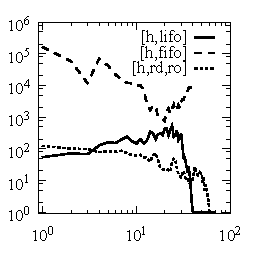
\includegraphics{tables/aaai16-log-rd/aaai16prelim3/depth-histogram-openstacks-opt11-strips-p10.pdf}
 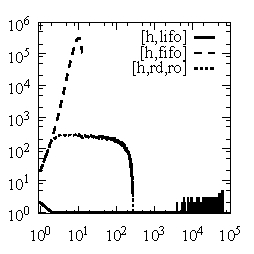
\includegraphics{tables/aaai16-log-rd/2zerocost/depth-histogram-woodworking-cut-p04.pdf}
 % 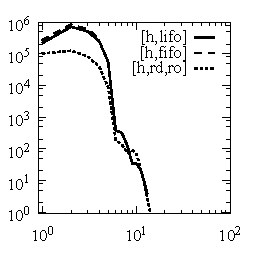
\includegraphics{tables/aaai16-log-rd/2zerocost/depth-histogram-psr-small-open-p48.pdf}
 }
 \caption{Number of nodes ($y$-axis) expanded per depth ($x$-axis) in
 the final plateau for 
 % (in left-to-right order)
 \pddl{Openstacks} p10 
 (left)
 and
 \pddl{Woodworking-cut} p04
 (right)
 %  and
 % \pddl{psr-small-open} p48
 with different tiebreakings.
 % Axes are logarithmic.
 }
 \label{fig:depth-histogram}
\end{figure}

\subsubsection{Comparison With $\varepsilon$-Cost Transformation}

\begin{table}[tb]
 \centering
 \begin{tabular}{|c|c|c||c|c|}
  \hline
  Domain & $[h,\fifo]/\varepsilon$ &  $[h,\lifo]/\varepsilon$ &  $[h,\fd,\ro]$ &  $[h,\rd,\ro]$ \\
  \hline
  \lmcut Zerocost & 261 & 259 & 257.4\spm{}2.0  &  \textbf{294.2\spm{}2.3} \\
  \hline
  \mands Zerocost & 282 & 282 & 274.0\spm{}0.9  &  \textbf{310.2\spm{}2.1} \\
  \hline
 \end{tabular}
 \caption{Comparison of  depth-based tiebreaking methods vs. standard $[h,\fifo]$ and $[h,lifo]$ methods applied to $\varepsilon$-cost-transformed versions of the problem instances}
 \label{tbl:epsilon}
\end{table}

An alternative approach to addressing the large plateaus in zero-cost domains is
to eliminate plateaus by introducing artificial gradients in the search space.
For example, the cost of all zero-cost actions can be replaced by a small $\varepsilon\ll 1$, where 
$\varepsilon$ is chosen such that the optimal cost for the result of  this \emph{$\varepsilon$-cost transformation} (``$\varepsilon$-transformation'') is the same as the cost of the optimal solution to the original domain with zero costs when the $\varepsilon$-transformed costs are mapped back to 0.

We evaluated the $[h,\fifo]/\varepsilon$ and $[h,\lifo]/\varepsilon$ strategies, which are the standard $[h,\fifo]$ and $[h,\lifo]$ tiebreaking strategies applied to  the $\varepsilon$-transformed version of the problems.
Since Fast Downward  only supports integer costs, we implemented/simulated the transformation by multiplying the non-zero costs by $10^6$, and assigning cost 1 to zero-cost actions -- in effect,  $\varepsilon=10^{-6}$.
\reftbl{tbl:epsilon} shows that $[h,\fifo]$ and $[h,\lifo]$ with $\varepsilon$-transformation
 perform comparably to $[h,\fd,\ro]$, but are outperformed by $[h,\rd,\ro]$.
% 
The similarity in performance between $\varepsilon$-transformation and $[h,\fd,\ro]$ can be explained by the fact that  OPEN is sorted according to  $f(n)+k(n)\varepsilon$,
where $k(n)$ is a number of zero-cost actions in the path to node $n$,
while expansion order of FirstDepth is equivalent to $f(n)+\depth{n}\varepsilon$.
($\depth{n}\leq k(n)$ because $k(n)$ accounts zero-cost actions also in non-final plateaus).
% 
One advantage of the $\varepsilon$-transformation is that it can be implemented by transforming the input problem and does not require implementation of depth-based buckets in the search algorithm.
On the other hand, there are two issues with the $\varepsilon$-transformation:
(1) $\varepsilon$ must be chosen carefully -- admissibility is lost  when $k(n)\varepsilon\approx 1$, and
(2) the number of possible $g$ and $f$ values becomes very large, making it difficult to use efficient $O(1)$ array-based implementation of the OPEN list and requiring the use of a heap-based $O(\log n)$ OPEN list.
% it makes array-based $O(1)$ OPEN-list consume too much memory
% because the queue contains too many different key values, 
% or it forces
% In contrast, depth can be directly implemented with just another level of nested arrays.



\section{Domain Configuration and Tiebreaking}
%Moved this out of the depth-based evaluation section because we also evaluate [h,fifo] and [h,lifo], and the results show that all are robust wrto action ordering
Recently, \citeauthor{vallati2015effective} showed that the performances of 
satisficing planners were significantly affected by PDDL domain \emph{configurations}, which include the name/ordering of actions, propositions, and objects in the PDDL input file (\citeyear{vallati2015effective}).
% note that vallati et al. did not show that tiebreaking was affected -- they observed that performance of the planners was affected by configuration, and conjectured that the performance variation was due to the effects of configuration on tiebreaking.
They conjectured that performance variations caused
by different domain configurations are due to the impact that the naming/ordering of objects has on tiebreaking.
% in \cite{vallati2015effective} p.7, col2, par#1
In Fast Downward, action names can affect search performance, because FD 
sorts the action schemas according to the dictionary
order of the schema names, which affects the order of applicable ground
actions, which in turn affects the node insertion order into OPEN.

%%%%%%%%%%%%%%%%%%%%%%%%%%%%%%%%%%%%%%%%%%%%%%%%%%%%5

We tested the robustness of the standard $[h,\lifo]$ and $[h,\fifo]$ strategies, as well as $[h,\rd,\ro]$,
with respect to 
biases introduced by domain configuration (action naming) in the PDDL domain definition.
We created 3 different sets of domains in which the
original names of action schema are mangled into random strings. 
%We only reordered the actions because in the FD codebase, the order of propositions has no effect on tiebreaking. --- let's avoid talking about anything other than action names, in case there are other configuration factors.
%  XXXTODO CHECK whether above sentence correctly summarizes the sentence below.
%% In contrast, we continued to use the variable ordering in the original domains
%% because the effect of variable ordering is irrelevant to the tiebreaking
%% criteria.
% %We avoided the effect of action orderings by using the randomized third tiebreaking.
%Each set of action-renamed domains contains all of the benchmark and zerocost domains.   %XX - can be inferred from table
We ran each of the 3 strategies on each
set of mangled domains, three times each with different random seeds,
resulting in 9 runs per strategy (recall that robustness wrto random seed was shown in \refsec{sec:depth-based-evaluation}.)

The results are shown in \reftbl{actionordering-robustness} (We
also included the original 10 runs from  \reftbl{depth}).
We statistically analyzed the results for $[h,\rd,\ro]$ 
to see if any of the 4 sets of domains
significantly outperformed the others.
%In order to test the significance of mean value,
Fligner-Killeen's non-parametric test could not reject the homogeneity of variances
($p=0.75$ for IPC, $p=0.26$ for Zerocost), so
% Since the variances were not significantly different,
we then applied the non-parametric Kruskal-Wallis test,
% to see if there is any difference in the mean values between the original
% population of the sample groups, 
which showed that the mean differences were not significant
($p=0.28$ for IPC, $p=0.44$ for Zerocost),
% We first applied Fligner-Killeen's non-parametric test to see if the sample groups 
% in each set of randomized domains share the same variance, 
% but could not reject the homogeneity of variances ($p=0.74$).
% Since the variances were not significantly different,
% we could then apply the non-parametric Kruskal-Wallis test to see if
% there is any difference in the mean values between the original
% population of the sample groups, which showed that the differences were not significant ($p=0.26$),
i.e., action name mangling did not significantly affect performance.

Thus, in contrast to the results for satisficing search by \cite{vallati2015effective}, 
the effect of action ordering  seems to be relatively weak for cost-optimal search using \astar.
This may be because 
compared to the satisficing, best-first search algorithms evaluated in \cite{vallati2015effective},
the behavior of admissible search is more constrained.
% $[h,\lifo]$, $[h,\fifo]$, and $[h,rd,\ro]$ are
% because of the first-level tiebreaking according to $h$.
%in that all nodes with cost $f$ must be expanded before any nodes with cost larger than $f$.
% this is true for best-first-search in general, by definition.

\begin{table}[tb]
 \setlength{\tabcolsep}{0.2em}
 \centering \relsize{-1}
 \begin{tabular}{|c|c|c||c|}
\hline         
 Domain & $[h,\fifo]$ & $[h,\lifo]$   & \spc{$[h,\rd,\ro]$ \\($n$: number of runs)}    \\
\hline         
 Mangled IPC 1 (1104) &  556 &  564 &  571.7\spm{}0.9 ($n=3$)\\\hline
 Mangled IPC 2 (1104) &  557 &  568 &  571.3\spm{}0.9 ($n=3$)\\\hline
 Mangled IPC 3 (1104) &  557 &  568 &  573.0\spm{}1.6 ($n=3$)\\\hline
 Original IPC (1104) &  558 &  565 &  570.6\spm{}1.5 ($n=10$)\\\hline
 Mangled Zerocost 1 (620) &  256 &  277 &  288.7\spm{}3.7 ($n=3$)\\\hline
 Mangled Zerocost 2 (620) &  256 &  277 &  285.0\spm{}0.8 ($n=3$)\\\hline
 Mangled Zerocost 3 (620) &  256 &  279 &  286.7\spm{}0.9 ($n=3$)\\\hline
 Original Zerocost  (620) &  256 &  279 &  287.2\spm{}2.4 ($n=10$)\\\hline
\end{tabular}

 \caption{Total coverages of $[h,\fifo]$, $[h,\lifo]$
 and $[h,\rd,\ro]$ (with three seeds). Each row represents the original set of
 domains or its three action-mangled variants. The effect
 of action ordering is small enough for $[h,\rd,\ro]$ to
 constantly perform better than the traditional tiebreaking methods.}
 \label{actionordering-robustness}
\end{table}

\section{Related Work}
\label{sec-4}

Previous work on escaping search space plateaus has focused on
non-admissible search.  DBFS \cite{imai2011novel} % is a technique which
adds stochastic backtracking to Greedy Best First Search (GBFS) to avoid
being misdirected by the heuristic function. Type based bucket
\cite{xie14type} classifies the plateau of GBFS according to the
$[g,h]$ pair and distributes the effort.  Marvin \cite{Coles07} learns plateau-escaping macros
from the Enhanced Hill Climbing phase of the FF planner
\cite{Hoffmann01}, and the use of these macros is inadmissible.
\citeauthor{Hoffmann05} gives a detailed analysis of the
structure of the search spaces of satisficing planning (\citeyear{Hoffmann05,Hoffmann11}).
\cite{benton2010g} proposes inadmissible technique for temporal planning
where short actions 
% are hidden behind long actions and
do not increase makespan. 
\cite{cushing2010cost} investigates ``$\varepsilon$-cost
traps''($\varepsilon=\frac{\min cost}{\max cost}$),  showing that (non-admissibly) treating all actions as unit cost sometimes finds an optimal plan quickly.
\cite{wilt2011cost} also analyzes inadmissible distance-to-go estimates.
% 
To our knowledge, 
plateaus have not been previously investigated for cost-optimal planning with admissible search.
Admissible and inadmissible search differ significantly in how non-final plateaus (plateaus with $f < f^*$) are treated:
Inadmissible search can skip or escape plateaus whenever possible, while
admissible search cannot, unless it
is the final plateau ($f=f^*$, $h=0$) and a solution is found. %it directly finds a solution.

%In their work on combining multiple heuristics in a planner, 
% \citeauthor{RogerH10} (\citeyear{RogerH10}) considered a tiebreaking approach which works as follows:
% When combining two heuristics, one of the
% heuristics is used as the primary criterion, % for guiding the search,
% and the second heuristic is used to break ties among nodes with the same primary
% heuristic value.
% While this did not perform well in their work on satisficing planning, 
% additional policy using a secondary heuristic
% for cost-optimal search is an interesting direction for future work.


The PLUSONE %\footnote{This term is used on the Fast Downward website.} XXfootnote takes too much space
cost-type (or distance-to-go) is a non-admissible search technique in the Fast Downward/LAMA planner
\cite{richter2010lama} which increases all action costs by 1.
% By eliminating zero-cost actions, this behaves similar to our $[h,\fd,\ro]$ tiebreaking.
%Using PLUSONE, three successive
%applications of zero-cost operators have cost 3, and two
%applications have cost 2, and smaller cost is preferred, just as
%\astar always expands the node with smaller $f$-value.
This technique explicitly targeted zero-cost actions,
and resulted in significantly better performance in the IPC-6
satisficing track \cite[p.137, Sec. 3.3.2]{richter2010lama}.
%\todo*{citation}
% There's a long discussion of Openstacks in \cite{richter2010lama}, p.167-169, but I can't find PLUSONE anywhere. Maybe it's called something else in the paper?  Maybe \richter2010lama is the wrong citation??
Unlike PLUSONE, depth-based tiebreaking is admissible.
%because unlike PLUSONE, action costs are not modified.  
Also, unlike PLUSONE, depth-based tiebreaking does not necessarily favor smaller depth over larger depth.
LAMA prefers smaller cost (including the increased cost),
which biases the search toward nodes with fewer zero-cost actions on their path.
This bias is similar to the $[h,\fd,\ro]$ policy,
the worst performer among all depth-variants in our experiments (\reftbl{depth}).
The best depth-based methods are  $[h,\ld,\ro]$ and $[h,\rd,\ro]$,
which do not prefer smaller depth.

% It's not clear what these techniques have in common, except that they are all orthogonal to heuristics,
% If that's the case, then there's no need to cite them in this paper -- there's no reason why these particular techniques
% are more relevant to this paper than hundreds of other techniques that are orthogonal to heuristics.
%% In admissible planning,
%% \emph{Symmetry Breaking}
%% \cite{Fox1998,pochter2011exploiting,domshlak2013symmetry} is the search
%% technique that tries to prune the states with symmetric
%% paths. \emph{Partial Order Reduction}
%% % , \emph{Strong Stubborn Sets} and \emph{Expansion Core} are
%% is also a technique which prunes the
%% intermediate states that reach to the same goal using the different
%% orders of same actions. \emph{Dominance Pruning} \cite{hall2013faster} is a
%% technique which prunes a state if it can be proven to be worse than the other nodes.
%% % 
%% These are usually not considered an attempt to improve the heuristic
%% estimates, however, in terms of \emph{Path-dependent globally admissible
%% heuristics} \cite{karpas2012optimal}, a class of heuristics which is
%% admissible only on a particular optimal path, generalizes the above
%% techniques as assigning an infinite cost to some nodes on the other optimal paths.
%% % 
%% % From a slightly different category, Pathmax \cite{mero1984heuristic} and
%% % Bidirectional Pathmax \cite{felner2011inconsistent} are the techniques
%% % which converts an inconsistent heuristics into non-decreasing,
%% % consistent heuristics.
%% Thus, in a broad term, all of these methods are the
%% attempts to improve the heuristic estimates.
%% % Although in some particular
%% % case they may be able to return a perfect heuristics, they are still not
%% % always a perfect heuristics, implying that the plateau is unavoidable.
%% In contrast, our tiebreaking techniques aims specifically at the case
%% where the plateau is encountered and the planners are forced to run a
%% knowledge-free search.

%% $LA^*$ \cite{stern2010look} extends \astar by performing a
%% cost-bounded depth-first \emph{lookahead} from each node as it is generated.
%% Under the lookahead cost bound $k=0$ ($LA^*_0$ in their notation),
%% all children with the same $f$-value are expanded.
%% The tiebreaking among the same $f$ is not documented either
%% in its main $A^*$ expansion nor in its DFS lookahead.


\section{Conclusion}

In this paper, we evaluated standard tiebreaking
strategies for \astar.
We showed that contrary to conventional wisdom, tiebreaking based on the heuristic value is not necessary to achieve good performance, and proposed
a new framework for defining tiebreaking policies based on \emph{depth}.
We showed that a depth-based, randomized strategy $[h,\rd,\ro]$, which uses the heuristic value, but explicitly avoids depth and ordering biases present in previous methods,
significantly outperforms previous strategies on domains with zero-cost actions, 
including practical application domains with resource optimization objectives in the IPC benchmarks.
% and slightly outperforms previous strategies on benchmark problems without zero-cost actions.
%We have shown that our $[h,\rd,\ro]$ strategy is successful because the randomized depth bucket selection explicitly avoids the depth bias that was present in previous methods
The proposed approach is highly effective on domains where zero-cost actions create large plateau regions where all nodes have the same $f$ and $h$ costs
and the heuristic function provides no useful guidance.
% We argued that such domains arise naturally when considering resource optimization problems.
%It also avoids the effect of action ordering in the domain definition,
%providing a robust behavior.
 % when the distribution of optimal solutions is not uniform within the open list.
% We also showed that this nonuniform distribution still appears when we have almost-perfect % heuristics.
%% Our method differs from the pruning techniques because we do not prune
%% any states, nor from the other general improvements to the heuristic
%% accuracy because we just change the evaluation order within the same
%% $f$, yet it address the fundamental problems in the heuristic forward
%% search. 
%% % 


%While we focused on randomized policies because plateaus, by definition do not provide useful heuristic information, 
%a direction for future work is development of deterministic variants.

%% not much details of the idea were presented in this paper. Also, I
%% don't want it to be copied by someone;;
% on-line adaptation methods that exploit search space neighborhood structure
% in order to adjust the tiebreaking policies.

\section{Tiebreaking Stratefy for GBFS}

\label{sec:gbfs}


